\scanpage{118}
\mspage{109}
% archive sheet number: 118 (lower left)
% L1-4
2) Pour tout support constructible $S\inserted{\deleted{\unsure{S}}\Phi}$ il existe un plus petit support constructible fermé le contenant, \inserted{si $S=\operatorname{supp}^{\circ}\Phi$,} il est donné par
\[
S=\operatorname{supp}^{\circ}(\overline{\Phi})=\operatorname{supp}(\overline{\Phi})
\]
% slanted
\margin{À vérifier ! Facile : c'est aussi $\operatorname{supp}^{\circ}(\widetilde{S})$ \unsure{\{} et $=\unsure{\operatorname{sat.}|\operatorname{sat}}\widetilde{S}$ adhérence au sens de la \unsure{rel.} $\unlhd$ de $\unsure{M|\mathcal{M}}$\unsure{.}}
% L5-7
--- mais \unsure{ici on fera|on fera} attention que \deleted{\unsure{$=$ si $\Phi$}} $\overline{\Phi}$ peut fort bien être morcelée, même si $\Phi$ ne \deleted{\unsure{$S$}} l'est pas.

% left margin drawing, slanted in the manuscript
\figure{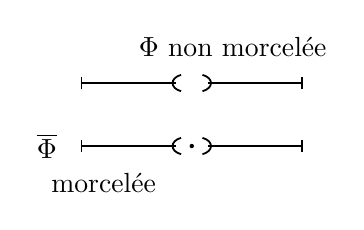
\begin{tikzpicture}[line width=.65pt,scale=.8]
\node at (2.4,.58) {$\Phi$ non morcelée};
\draw (0,0)--(1.5,0); \draw (2,0)--(3.5,0);
\draw (0,-.1)--(0,.1); \draw (3.5,-.1)--(3.5,.1);
\draw (1.58,.13) .. controls (1.40,.08) and (1.40,-.08) .. (1.58,-.13);
\draw (1.92,.13) .. controls (2.10,.08) and (2.10,-.08) .. (1.92,-.13);
\node at (-.55,-1) {$\overline{\Phi}$};
\draw (0,-1)--(1.5,-1); \draw (2,-1)--(3.5,-1);
\draw (0,-1.1)--(0,-.9); \draw (3.5,-1.1)--(3.5,-.9);
\draw (1.58,-.87) .. controls (1.40,-.92) and (1.40,-1.08) .. (1.58,-1.13);
\draw (1.92,-.87) .. controls (2.10,-.92) and (2.10,-1.08) .. (1.92,-1.13);
\fill (1.75,-1) circle (.035);
\node at (.35,-1.58) {morcelée};
\end{tikzpicture}}
% L8-10
3) Description combinatoire des supports constructibles via les préfigures non morcelées\textsuperscript{*}

% L11-17
\uline{4. juillet} Je voudrais donner une \unsure{paramétrisation} tant soit peu ``autoduale'' des supports constructibles, i.e. des préfigures non morcelées (ou ``\unsure{irredondantes|irrédondantes}''). Pour cela il faut ``mettre à part'' ses points isolés\inserted{de $\Phi$}, et les traiter en vis-à-vis des points de $\unsure{\mathcal{L}|L}$ qui \deleted{sont} ne sont pas dans $\Phi$, mais adhérents à $\Phi$ dans $M$\textsuperscript{\(\unsure{\lambda}\)}.
% slanted
\margin{$\unsure{\lambda}$ et \deleted{\unsure{pas}} $\notin\unsure{\partial|\delta}\Phi$ --- i.e. les ``points-frontière internes''}

On trouve ceci.

% L18-24
On regarde la figure \deleted{$\Phi_1=$} \deleted{$\overline{\Phi}\setminus\text{ens des points isolés}$} \deleted{de $\overline{\Phi}$}
\[
\Phi_1=\overline{\Phi}\setminus\{\text{ens des points isolés de }\overline{\Phi}\}
\]
c'est une figure qui \deleted{\unsure{n'est p}} peut ou pas être \unsure{irredondante|irrédondante}. Celle l'est sss \deleted{$\Phi$} \deleted{\unsure{ou|si} \unsure{que des|des} $\deleted{\unsure{\Phi}}\overline{\Phi}\setminus\Phi$ est formé de points de}
\[
\overline{\Phi}\setminus\Phi\subset\partial\Phi=\{s\in\delta\Phi\mid\text{ordre de }s\text{ dans }\overline{\Phi}\text{ est }1\}
\]
i.e. sss $\Phi$ n'a \deleted{\unsure{$\Phi$}} pas de point frontière interne
